\documentclass[12pt]{article}
\usepackage{amssymb,amsfonts,amsmath,graphicx,mathtools}
\usepackage[alphabetic,y2k,lite]{amsrefs}
\usepackage{fullpage, mystyle}
\usepackage{MnSymbol}

\usepackage{tikz-cd}

\newcommand{\disk}[1]{{D^{#1}}}
\newcommand{\sphr}[1]{{S^{#1}}}
\newcommand{\empt}[1]{{\emptyset^{#1}}}

\begin{document}

\title{Upgrading an $(n+\veps)$-TQFT to an extended $(n+1)$-TQFT}
\author{Ying Hong Tham}
\maketitle


In this note, we show that one can promote an
$(n+\veps)$-TQFT to an extended $(n+1)$-TQFT
by only specifying the value associated to
the $(n+1)$-disk $Z(\disk{n+1}) \in Z(S^n)$.

Suppose we are given an $(n+\veps)$-TQFT $Z$,
that is,
it assigns a category $Z(N)$ to a closed $(n-1)$-manifold $N$,
and a functor $Z(M):Z(N) \to Z(N')$ to an $n$-dimensional
cobordisms $M:N\to N'$ between $(n-1)$-manifolds.

TODO perhaps comment on requirements on $Z$,
e.g. a natural isom for $M \simeq M'$,
especially for $Z(M' \circ M) \simeq Z(M') \circ Z(M)$
that is consistent.
Or say, at this point, no assumption on existence of
adjointness of functors $Z(M) \dashv Z(\ov{M})$.

The empty $k$-manifold is denoted by $\empt{k}$.
Composition of cobordisms is written from right to left,
so composition of $M: N \to N'$ and $M' : N' \to N''$
is denoted by $M' \circ M: N \to N''$.

\begin{proposition}
\label{p:extend-uniqueness}
Consider functors
$Z(\disk{n}) : Z(\empt{n-1}) \rightleftharpoons
	Z(\sphr{n-1}) : Z(\ov{\disk{n}})$.

Let $\eta_0: Z(\empt{n}) \Rightarrow
	Z(\sphr{n} = \ov{\disk{n}} \circ \disk{n})
	: Z(\empt{n-1}) \to Z(\empt{n-1})$
be a natural transformation,
and suppose it is the unit to an adjunction
$Z(\disk{n}) \dashv Z(\ov{\disk{n}})$.

Then if $Z',Z''$ are extended $(n+1)$-TQFTs
such that $Z',Z''$ agree with $Z$ on $(n-1)$- and $n$-manifolds,
and $Z'(\disk{n+1}) = Z''(\disk{n+1}) = \eta_0$,
then $Z' \cong Z''$.
\end{proposition}


The proof of this proposition occupies the rest of this article.



\subsection{Adjunctions from topology}

In the 2-category with closed $(n-1)$-manifolds as objects,
$n$-dimensional cobordisms as 1-morphisms,
and $(n+1)$-dimensional relative cobordisms as 2-morphisms,
the $n$-dimensional cobordisms
$M: N \rightleftharpoons N' : \ov{M}$
form an adjunction.

Let us first consider a simple case,
which is the main setting in \prpref{p:extend-uniqueness}.
Consider $n$-dim cobordisms
$\disk{n}: \empt{n-1} \rightleftharpoons
	\sphr{n-1}: \ov{\disk{n}}$.
This can be promoted to an adjunction
$\disk{n} \dashv \ov{\disk{n}}$
with the following unit and counit 2-morphisms:
the unit is given by the $(n+1)$-disk
$\disk{n+1}: \empt{n} \Rightarrow
	(\ov{\disk{n}} \circ \disk{n}) = \sphr{n}$,
and the counit is given by the $(n+1)$-disk which,
as a manifold with corner $\sphr{0} \times \sphr{n-1}$,
is a 2-morphism
$\disk{n+1} = I \times \disk{n}: \disk{n} \circ \ov{\disk{n}}
	\Rightarrow I \times \sphr{n-1} = \id_{\sphr{n-1}}$.
This is easily checked to be an adjunction,
the unit is an $(n+1)$-dimensional 0-handle,
and the counit is attaching an $(n+1)$-dimensional 1-handle
to $\disk{n} \sqcup \ov{\disk{n}}$
(see \figref{f:disk-adjunction} for $n=1$ case).

\begin{figure}[ht]
\rotatebox[origin=c]{180}{
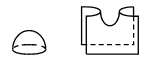
\includegraphics[width=6cm]{disk-adjunction-unit-counit.png}
}
\hspace{20pt};
\hspace{20pt}
\rotatebox[origin=c]{180}{
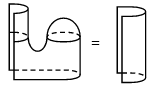
\includegraphics[width=6cm]{disk-adjunction-snake-equation.png}
}
\caption{Counit and unit for adjunction
$\disk{n}: \empt{n-1} \rightleftharpoons
	\sphr{n-1}: \ov{\disk{n}}$,
for $n=1$,
along with one of the snake equations;
relative cobordism goes up
(stolen from \cite{SPries},
Figure 1.6 and 1.10, get rotated)}
\label{f:disk-adjunction}
\end{figure}


Now consider $M: N \rightleftharpoons N': \ov{M}$,
where $M$ is an elementary cobordism of index $k$,
i.e. it is obtained from $N \times I$
by attaching a $k$-handle.
Then $\ov{M}$ is the dual elementary cobordism
which is of index $n-k$.
[See \figref{f:dual-handle}]

\begin{figure}[ht]
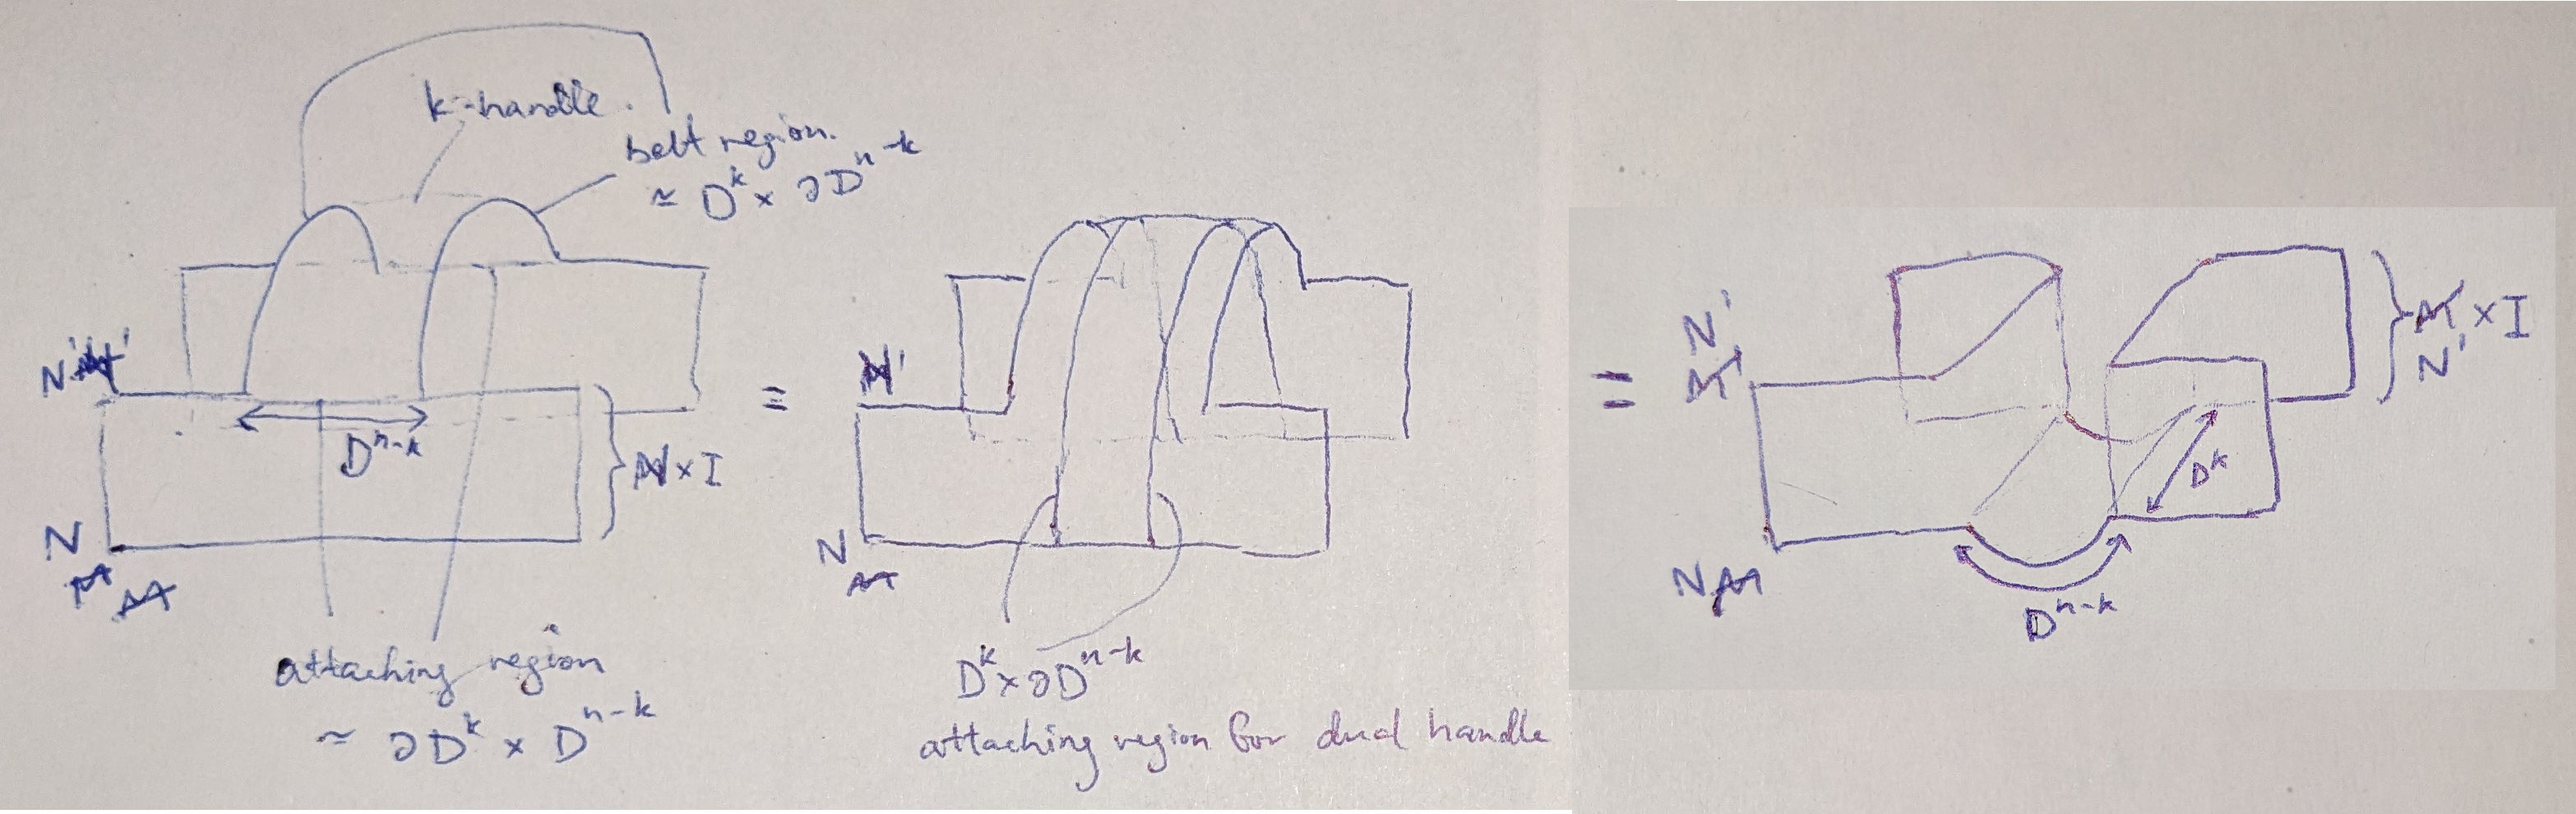
\includegraphics[width=15cm]{diagram-dual-handle.jpg}
\caption{$M:N \to N'$ is an elementary cobordism
of index $k$; it is built from attaching a disk $\disk{n}$
to $N \times I$,
with attaching region $\del \disk{k} \times \disk{n-k}$.
It can also be built from the other direction,
by attaching a disk $\disk{n}$
to $N' \times I$,
with attaching region $\disk{k} \times \del \disk{n-k}$.
Thus, turning it upside-down, i.e.
treated as a cobordism $\ov{M}: N' \to N$,
it is an elementary cobordism of index $(n-k)$.
}
\label{f:dual-handle}
\end{figure}

[See \figref{f:elementary-cobord-counit-unit}]
We construct the counit
$\veps: M \circ \ov{M} \Rightarrow \id_{N'} : N' \to N'$
by attaching an
$(n+1)$-dimensional $(k+1)$-handle to $M \cup_{N'} \ov{M}$,
with attaching region being essentially the
$k$-handle in $M$ plus the $(n-k)$-handle in $\ov{M}$;
the attaching sphere is the union of the core of the
$k$-handle in $M$
with the co-core of the $(n-k)$-handle in $\ov{M}$.
Similarly,
we construct the unit
$\eta: \id_N \Rightarrow M \circ \ov{M} : N \to N$
by attaching an
$(n+1)$-dimensional $k$-handle to $\id_N = N \times I$;
the attaching region for this $(n+1)$-dim $k$-handle
is
$($the attaching region for the $n$-dim $k$-handle that defines
$M) \times I$.
The snake equations
$\id_M = (\veps \circ M) \cdot (M \circ \eta):
M \Rightarrow M \circ \ov{M} \circ M \Rightarrow M$
and
$\id_{\ov{M}} = (\ov{M} \circ \eta) \cdot (\eta \circ \ov{M}):
\ov{M} \Rightarrow \ov{M} \circ M \circ \ov{M} \Rightarrow \ov{M}$
follow from the fact that
these $(n+1)$-dim handles form a cancelling pair
in both cases.

Here we have $M \dashv \ov{M}$,
but we may very well have $\ov{M} \dashv M$;
the counit $\veps': \ov{M} \circ M \Rightarrow \id_N$
is an $(n+1)$-dim elementary cobordism
of index $(n-k+1)$.
It is interesting to note that
this counit is the dual cobordism to the unit
$\eta: \id_N \Rightarrow \ov{M} \circ M$
previously described.

\begin{figure}[ht]
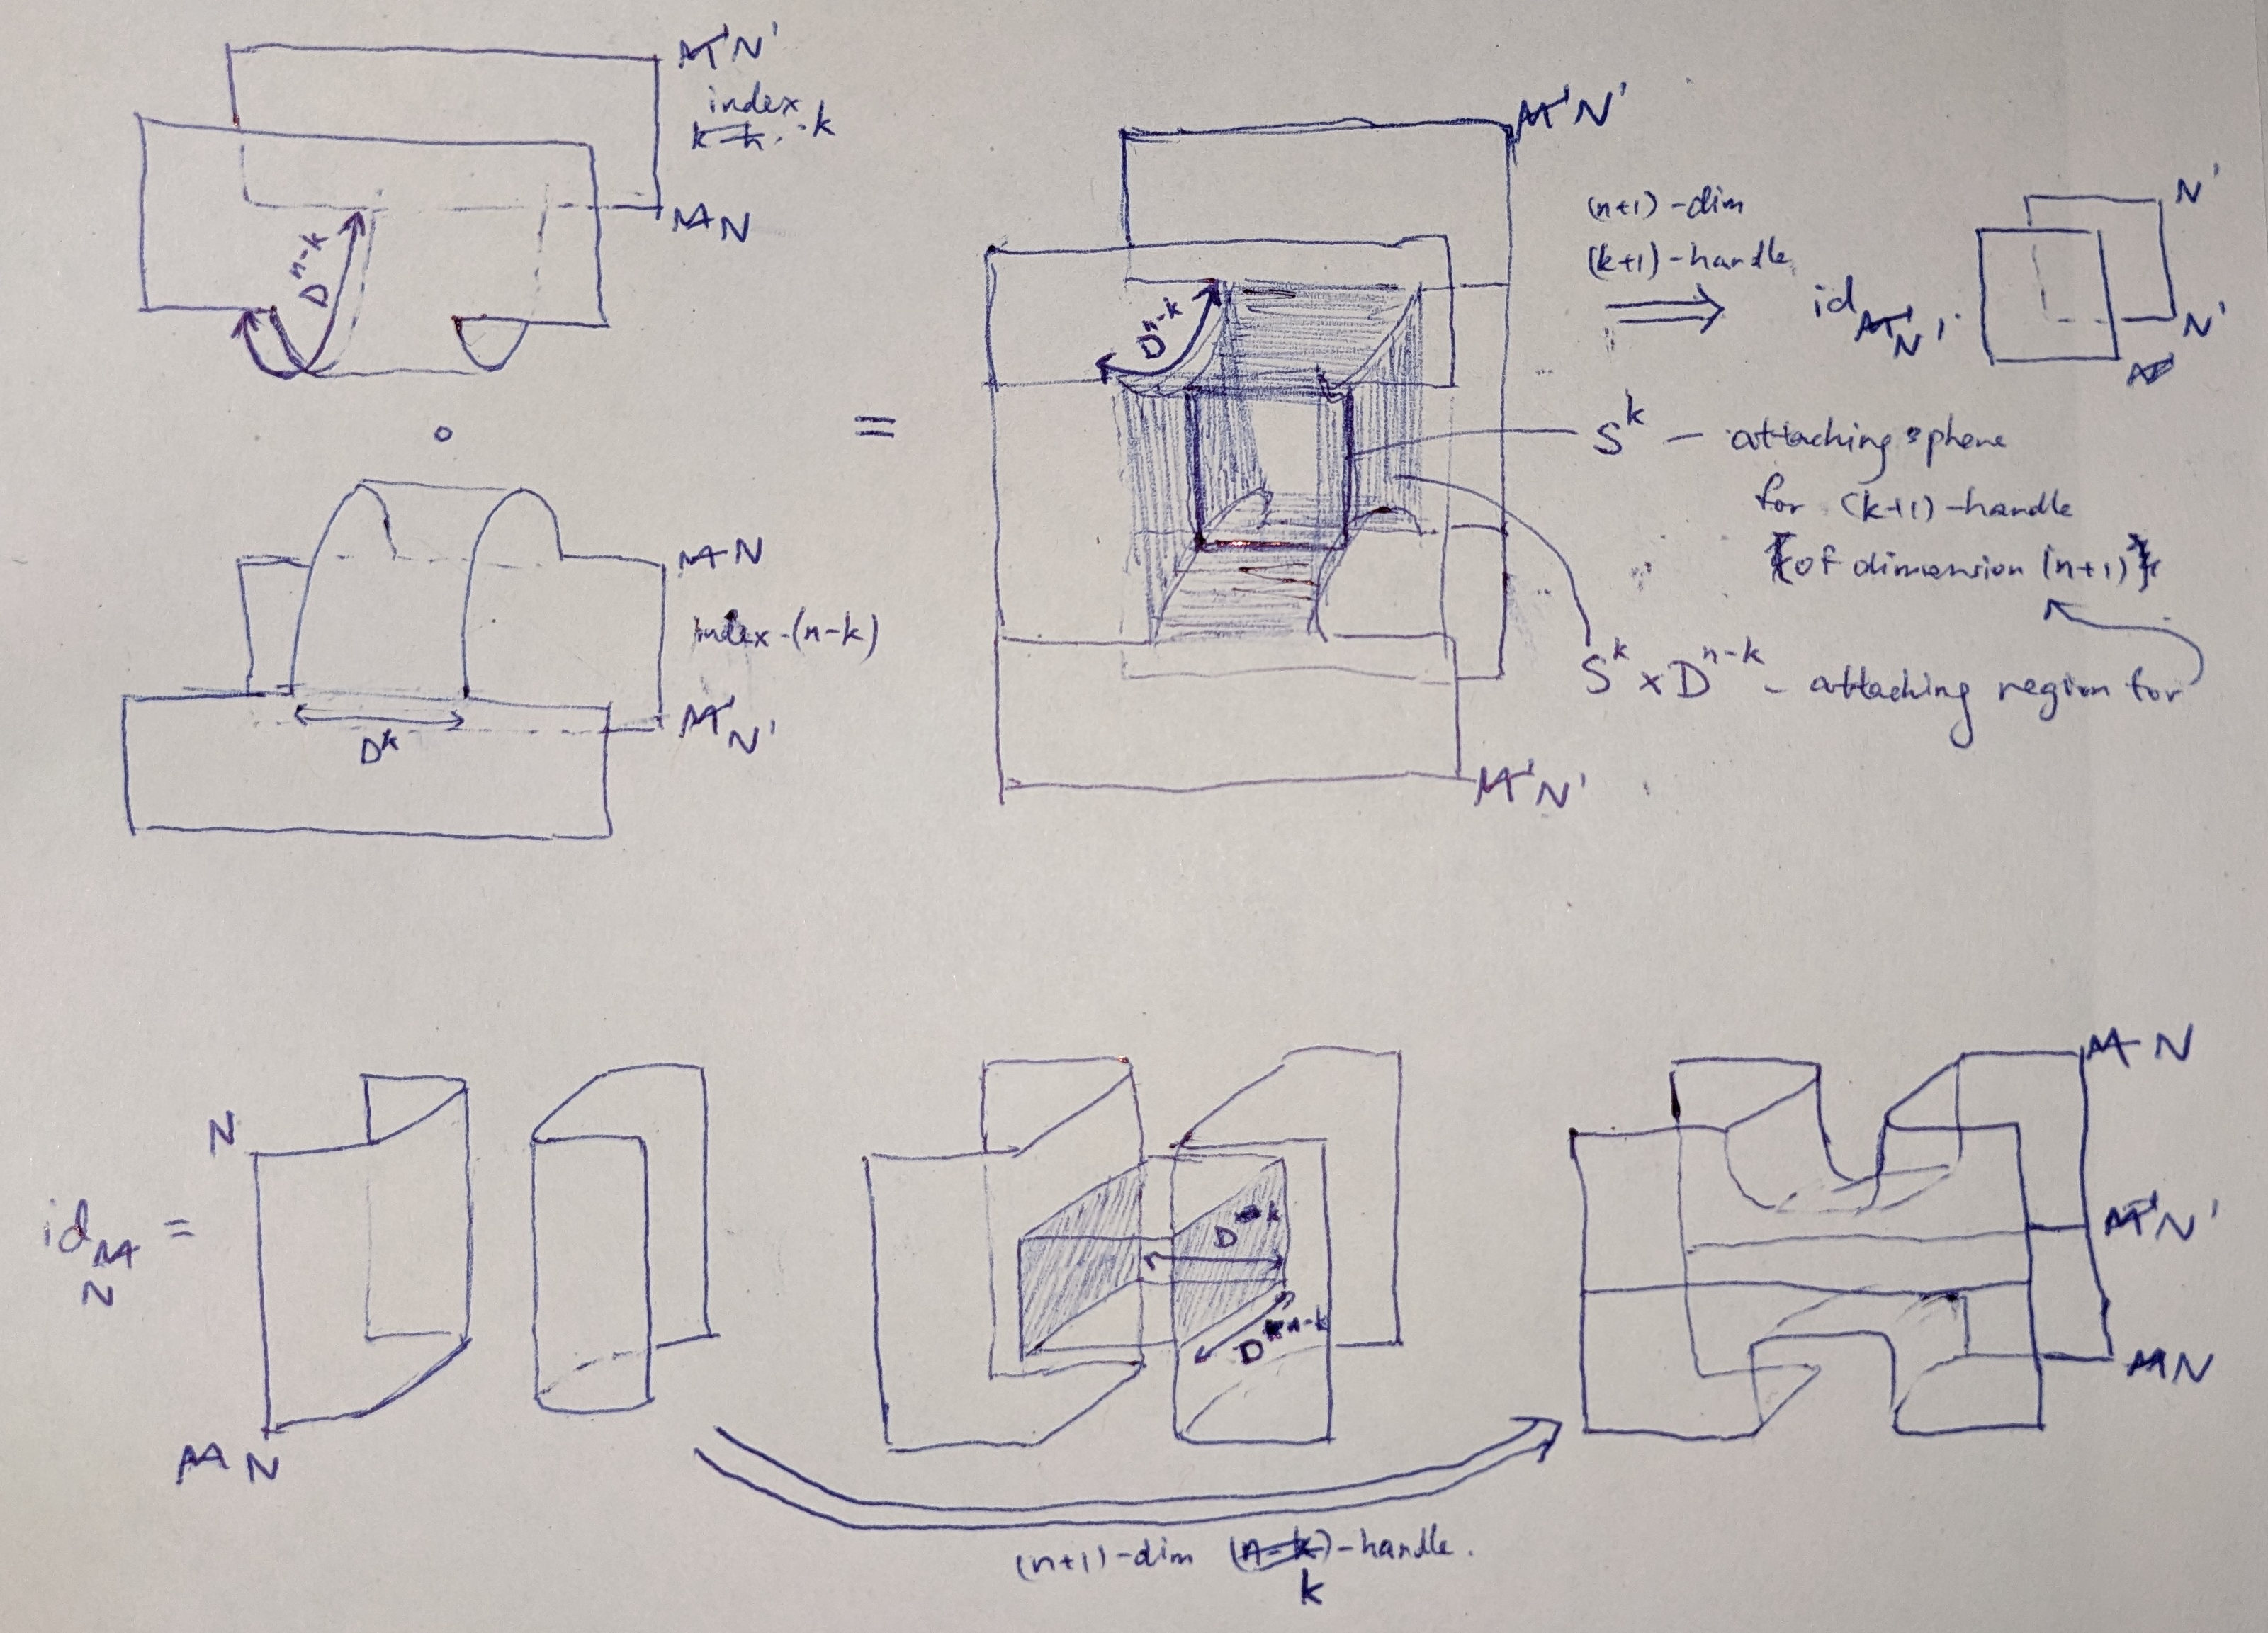
\includegraphics[width=15cm]{diagram-counit-unit-elementary-cobord.jpg}
\caption{Counit (top) and unit (bottom) for adjunction
$M: N \rightleftharpoons N': \ov{M}$,
where $M$ is an elementary cobordism of index $k$.
Note the way $N$ is drawn here looks like $N'$
in \figref{f:dual-handle} and vice versa
(by accident, sorry for minor confusion)}
\label{f:elementary-cobord-counit-unit}
\end{figure}



In general, we may consider the pair of $n$-dim cobordisms
$M : N \rightleftharpoons N': \ov{M}$.
By presenting $M$ as a composition of elementary cobordisms,
we may compose the adjunctions constructed
for each of these elementary cobordisms as above,
and obtain an adjunction $M \dashv \ov{M}$.



\begin{remark}
In \cite{Yprod},
we considered this construction
without realizing their connection to these adjunctions;
there we consider the more general case where
$N,N'$ may have (possibly different) boundary, and
$M: N \to N'$ is a relative cobordism
(with the boundary cobordism that is
not necessarily the identity cobordism).
\end{remark}


For our applications,
we will consider in detail the adjunction
$\empt{n-1} : \empt{n} \rightleftharpoons
	\sphr{k} \times \sphr{n-1-k} : \sphr{k} \times \disk{n-k}$.


\begin{thebibliography}{1}

\bibitem{Yprod} Kwon, Alice, and Ying Hong Tham. The Y-Product. arXiv preprint arXiv:2209.14251 (2022).

\bibitem{SPries} Schommer-Pries, Christopher John. The classification of two-dimensional extended topological field theories. University of California, Berkeley, 2009.

\end{thebibliography}


\end{document}
